\documentclass{homework}
\usepackage{graphicx}
\usepackage{booktabs}
\usepackage{amssymb,amsmath,latexsym,amsfonts,amsthm}
\usepackage{mathtools}
\usepackage{cleveref}
\usepackage{enumerate}
\setlength{\parskip}{1em} 



\studentname{Jiarong Zhu} % Your name here
\studentuni{jz2977} % Your UNI here
\coursename{COMS 4731 Fall 2019} % Course name
\homework{1} % Homework number
\date{September 18, 2019} % Date

\begin{document}
\maketitle
\setlength{\parindent}{0pt}

\section{Problem 1}
\begin{enumerate}[a)]
	\item Answer: Circle
	
	\item Answer: 0.25 mm$^2$
	
	Assume $r_{d}$ is the radius of the disk itself, $r_{i}$ is the radius of disk in the image, $d_{d}$ is the distance from the pinhole to the disk itself, $d_{i}$ is the distance from the pinhole to the image plane. We know that
$$
\frac{r_{d}}{d_{d}} = \frac{r_i}{d_i}$$

	Since the new distance from the pinhole to the disk itself $D_d = 2d_d$, the new radius of disk in the image $R_i$ will be 
\begin{align*}
R_i &= \frac{r_d}{D_d}d_i  \\
&= \frac{1}{2} \frac{r_d}{d_d}d_i \\
&= \frac{1}{2}r_i
\end{align*}

	Since the radius is half of the original radius, the area is 0.25 mm$^2$

	\item Answer: Ellipse. 
	
	Because the locus of the lines of sight
tangent to a sphere is a cone of revolution. The intersection of this cone of revolution with the image plane is the contour of the image of the sphere. If the sphere is one side of the image plane and the center of projection is on
the other side, the shape of the image pf the sphere can only be an ellipse or a circle (which is a special ellipse).

\end{enumerate}


\section{Problem 2}

\begin{enumerate}[a)]
	\item Answer: $\frac{kf}{k- f}$ when $k> f$
	
	\begin{align*}
	\frac{1}{f} &=\frac{1}{d} + \frac{1}{k} \\
	\frac{1}{d} &= \frac{k-f}{kf} \\
	d &= \frac{kf}{k-f}
	\end{align*}

	Since $d$ should be positive, only when $k > f$, the focused image of the scene line would be formed.
	
	\item Answer: 
	\begin{figure}[h!]
	\centering
  	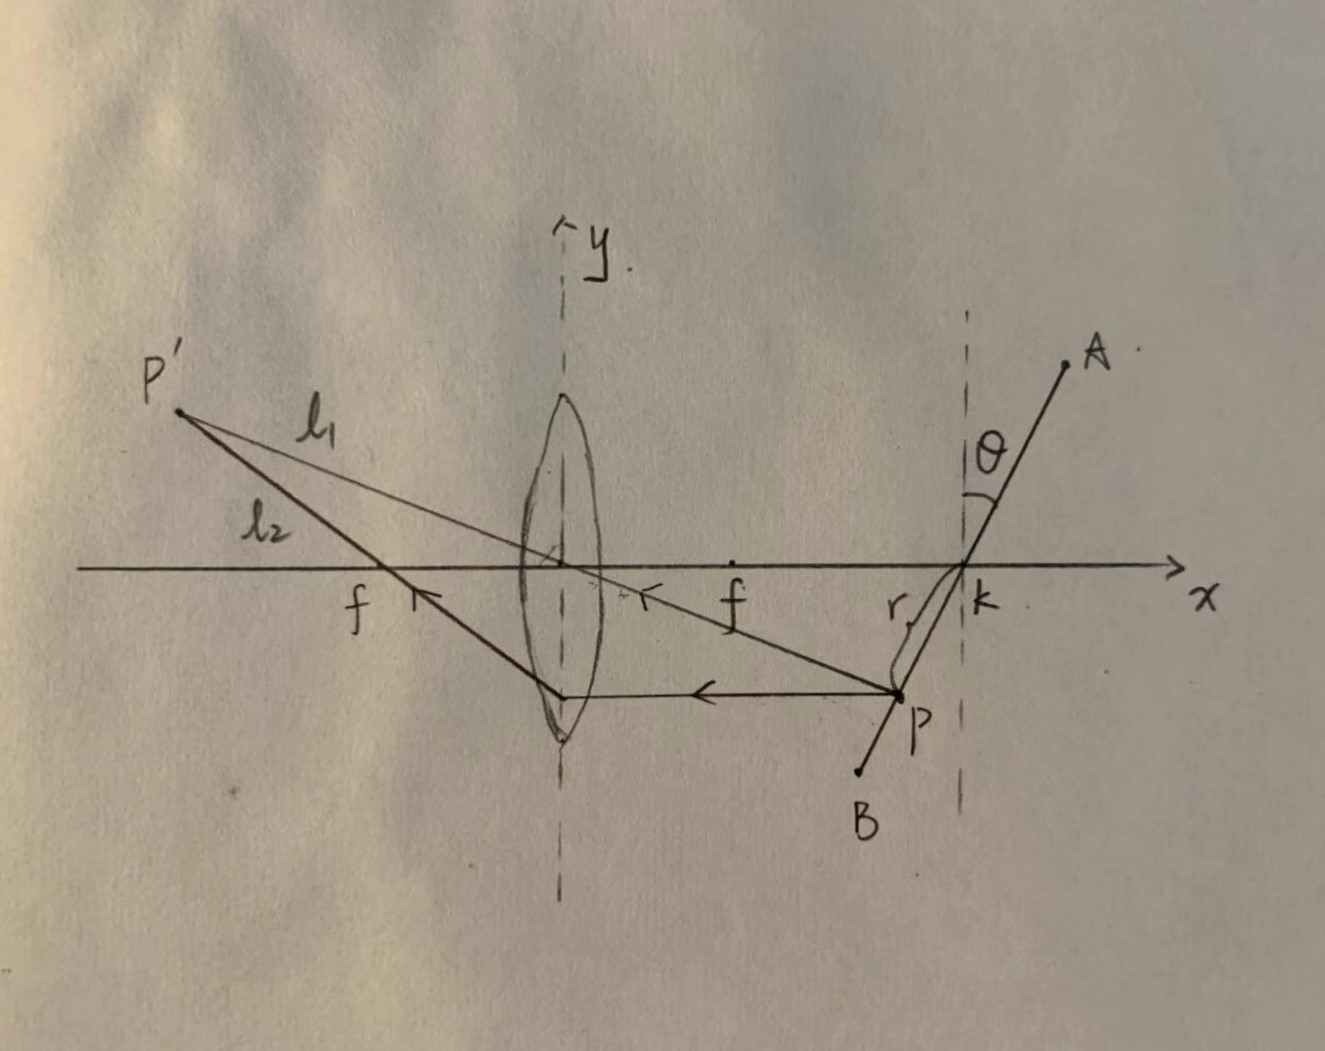
\includegraphics[scale=0.3]{p2b.jpg}
  	\caption{Coordinate system diagram}
  	\label{fig:p2b}
	\end{figure}
	
	Assume the coordinate system shown in Figure \ref{fig:p2b} was set up. $r$ is any real number which is less than $\frac{1}{2}AB$ and the coordinate of $P$ can be written as $(k-r\sin\theta, -r\cos\theta)$ \\
	
	The function of $l_1$: 
	\begin{equation}
	y=\frac{-r\cos\theta}{k-r\sin\theta}x\label{eq:1}
	\end{equation}
	
	The function of $l_2$: 
	\begin{equation}
	y=-\frac{r\cos\theta}{f}x-r\cos\theta\label{eq:2}
	\end{equation}
	
	Combine Equation \ref{eq:1} and Equation \ref{eq:2} and we can solve the coordinate of $P^{'}$:
	
	$$(\frac{k-r\sin\theta}{f-k+r\sin\theta}, \frac{-r\cos\theta}{f-k+r\sin\theta}), \quad r\in[0,\frac{1}{2}AB]  $$
	
	$P^{'}$ is on the line whose function is:
	
	$$y=\frac{f-k}{f\tan\theta}x-\frac{k}{f\tan\theta}$$
	
	So, we can prove that the image of the scene line is still a line. Since the slope is different from the slope of the original line, we can prove that it is tilted.
	
	\item Answer:
	
	From b) we can know the slope of the tilted scene is $\frac{f-k}{f\tan\theta}$ which is also equal to $\tan(\phi+\frac{\pi}{2})$
	
	So, we can prove that $\tan\phi = \frac{f}{k-f}\tan\theta$

\end{enumerate}

\section{Problem 3}

\begin{enumerate}[a)]

	\item Answer:
	
	We can generate the functions of $L_1$ and $L_2$ respectively:
	
	\begin{align*}
	L_1 = \frac{\rho_d I}{\pi r^2}(\overrightarrow{n} \cdot \overrightarrow{s_1})
	\end{align*}
	\begin{align*}
	L_2 = \frac{\rho_d I}{\pi r^2}(\overrightarrow{n} \cdot \overrightarrow{s_2})
	\end{align*}
	\begin{align*}
	L_3 &= L_1 + L_2 \\
	&= \frac{\rho_d I}{\pi r^2}\overrightarrow{n} \cdot (\overrightarrow{s_1}+\overrightarrow{s_2}) \\
	&= \frac{\rho_d }{\pi r^2}|\overrightarrow{s_1}+\overrightarrow{s_2}|I  \overrightarrow{n} \cdot \frac{(\overrightarrow{s_1}+\overrightarrow{s_2})}{|\overrightarrow{s_1}+\overrightarrow{s_2}|} 
	\end{align*}
	So,
	\begin{align*}
	s_3 &= \frac{(\overrightarrow{s_1}+\overrightarrow{s_2})}{|\overrightarrow{s_1}+\overrightarrow{s_2}|} \\
	I_3 &= |\overrightarrow{s_1}+\overrightarrow{s_2}| I
	\end{align*}
		
	\item Answer:
	
	\begin{align*}
	L_1 = \frac{\rho_d I_1}{\pi r^2}(\overrightarrow{n} \cdot \overrightarrow{s_1})
	\end{align*}
	\begin{align*}
	L_2 = \frac{\rho_d I_2}{\pi r^2}(\overrightarrow{n} \cdot \overrightarrow{s_2})
	\end{align*}
	\begin{align*}
	L_3 &= L_1 + L_2 \\
	&= \frac{\rho_d}{\pi r^2}\overrightarrow{n} \cdot (I_1 \overrightarrow{s_1}+I_2\overrightarrow{s_2}) \\
	&= \frac{\rho_d }{\pi r^2} |I_1 \overrightarrow{s_1}+I_2\overrightarrow{s_2}| \overrightarrow{n} \cdot 
	\frac{I_1 \overrightarrow{s_1}+I_2\overrightarrow{s_2}}{|I_1 \overrightarrow{s_1}+I_2\overrightarrow{s_2}|}
	\end{align*}
	So,
	\begin{align*}
	s_3 &= \frac{I_1 \overrightarrow{s_1}+I_2\overrightarrow{s_2}}{|I_1 \overrightarrow{s_1}+I_2\overrightarrow{s_2}|} \\
	I_3 &= |I_1 \overrightarrow{s_1}+I_2\overrightarrow{s_2}|
	\end{align*}
	
\end{enumerate}








\end{document}

